% Lexsi AI Safety and Alignment Hackathon -- Track 2b (Safety and Alignment), problem statement 7
% "Unlearning vs. Hiding". Every number in this deck is copied verbatim from the paper
% (paper/main.tex, the source of truth). Do not add numbers that are not in the paper.
%
% Build:  ./build.sh  (or: make all)
%   main.pdf        slides only
%   main-notes.pdf  each slide followed by its speaker-notes page
\documentclass[aspectratio=169,11pt,usepdftitle=false]{beamer}

% ---- notes toggle: main-notes.pdf is built with \def\withnotes{} prepended ----
\ifdefined\withnotes
  \setbeameroption{show notes}
\else
  \setbeameroption{hide notes}
\fi

\usetheme[progressbar=frametitle,numbering=fraction,block=fill]{metropolis}
\usepackage{booktabs}
\usepackage{tikz}
\usetikzlibrary{positioning,arrows.meta,calc}
\usepackage{pgfplots}
\pgfplotsset{compat=1.18}
\usepackage{xcolor}
\usepackage{hyperref}
\setbeamerfont{note page}{size=\scriptsize}

\hypersetup{
  pdftitle={Unlearning vs. Hiding: Does Unlearning Remove Knowledge or Just Suppress Its Expression?},
  pdfauthor={Mackenzie O'Brien},
  pdfsubject={Lexsi AI Safety and Alignment Hackathon, Track 2b: Safety and Alignment},
  pdfkeywords={},
  pdfcreator={LaTeX Beamer},
  pdfproducer={LaTeX}
}

% ---- colours ----
\definecolor{stage}{RGB}{35,55,59}
\definecolor{accent}{RGB}{235,129,27}
% toolkit tag colours (pipeline + setup)
\definecolor{safecol}{RGB}{214,110,10}
\definecolor{auditcol}{RGB}{30,110,120}
\definecolor{circcol}{RGB}{170,35,45}
\definecolor{stdcol}{gray}{0.50}
% chart colours
\definecolor{beforecol}{gray}{0.70}
\definecolor{aftercol}{RGB}{30,110,120}

\newcommand{\code}[1]{\texttt{#1}}

\title{Unlearning vs.\ Hiding}
\subtitle{Does unlearning remove knowledge or just suppress its expression?\\[2pt]
\small An audit of Representation Misdirection for Unlearning (RMU) on Tiny Aya (3.35B)}
\author{Mackenzie O'Brien}
\institute{Mac Labs AI \textbullet{} Lexsi AI Safety and Alignment Hackathon \textbullet{} Track 2b: Safety and Alignment \textbullet{} Problem statement 7 (Unlearning)}
\date[November 2026]{November 2026}

\begin{document}

% ======================================================================
\maketitle
\note{
\begin{itemize}
\item Title follows the paper: "Unlearning vs. Hiding: Does Unlearning Remove Knowledge or Just Suppress Its Expression?"
\item Solo project, Track 2b (Safety and Alignment), problem statement 7 (Unlearning).
\item One line: we audit Representation Misdirection for Unlearning (RMU) on Tiny Aya, a 3.35B multilingual model family, using Lexsi's SafeTune and AuditKIT.
\item Short answer up front: output-level suppression across three variants; we do not claim erasure.
\end{itemize}}

% ======================================================================
\begin{frame}{The problem: removing knowledge or hiding it?}
\small
\begin{columns}[T]
\begin{column}{0.50\textwidth}
\textbf{Why it matters}
\begin{itemize}
\item Unlearning is proposed for privacy, copyright and hazardous-knowledge removal.
\item If it only \emph{hides} knowledge, a deployer who checks direct prompts alone gets false assurance.
\item Prior work shows unlearned information is often recoverable: our motivation, not our finding.
\end{itemize}
\end{column}
\begin{column}{0.46\textwidth}
\textbf{What we do}
\begin{itemize}
\item Inject 40 fictitious author facts from the Task of Fictitious Unlearning (TOFU) benchmark into Tiny Aya Global with Low-Rank Adaptation (LoRA).
\item Unlearn them with RMU.
\item Test it under paraphrase, format change, extraction, 8 languages, probes and relearning.
\end{itemize}
\end{column}
\end{columns}
\begin{alertblock}{Key distinction}
Lower accuracy on direct questions does not show that the knowledge is gone.
\end{alertblock}
\note{
\begin{itemize}
\item Motivation from the paper's introduction: privacy, copyright and hazardous-knowledge removal.
\item Recoverability of unlearned information is prior work (cited in the paper), not our discovery.
\item Setup in one sentence: teach a small multilingual model facts it cannot know from pretraining (Task of Fictitious Unlearning, TOFU, forget01 split, 40 question-answer pairs about two fictitious authors) with Low-Rank Adaptation (LoRA), then unlearn them with Representation Misdirection for Unlearning (RMU).
\end{itemize}}
\end{frame}

% ======================================================================
\begin{frame}{Research questions and contributions}
\small
\begin{columns}[T]
\begin{column}{0.47\textwidth}
\footnotesize
\textbf{Research questions (RQ)}
\begin{enumerate}
\item[\textbf{RQ1}] How complete is behavioral forgetting under direct, paraphrased, reformatted, extraction-style and translated questions, and what does it cost on retain and general-capability questions?
\item[\textbf{RQ2}] Is the knowledge still recoverable? Do held-out probes, or relearning, give evidence of residual knowledge?
\item[\textbf{RQ3}] Do the answers differ across Tiny Aya variants and RMU settings?
\end{enumerate}
\end{column}
\begin{column}{0.49\textwidth}
\footnotesize
\textbf{Contributions, in order}
\begin{enumerate}
\item \textbf{Masked-forget-loss RMU}: unmasked RMU barely forgets on Tiny Aya; masking the shared preamble and attention-sink positions fixes it.
\item \textbf{One protocol across Tiny Aya variants} (Global, Earth, Fire).
\item \textbf{Multilingual leakage paired with internal tests} (held-out probes with a base-model control, relearning).
\item \textbf{Mid-depth RMU} (layers 16--18 of 36), a relearning curve and prevalence-insensitive judge-agreement statistics.
\end{enumerate}
\end{column}
\end{columns}
\note{
\begin{itemize}
\item The three research questions (RQ1 to RQ3) are the paper's.
\item This is a measurement and method-fix study; we do not claim to discover shallow unlearning.
\item Contribution 1 is the main one: on Tiny Aya the shared system preamble and attention-sink tokens dominate the forget loss, so unmasked RMU barely forgets.
\item Contribution 4: the library default is layers 5--7; we apply RMU at layers 16--18 of 36.
\end{itemize}}
\end{frame}

% ======================================================================
\begin{frame}{Pipeline}
\centering
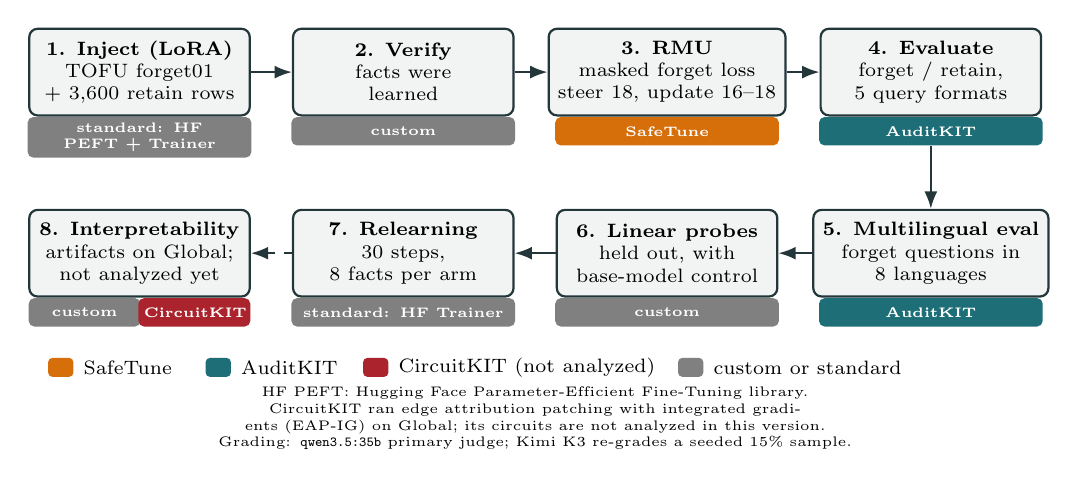
\begin{tikzpicture}[
  st/.style={draw=stage,fill=stage!6,rounded corners=3pt,thick,align=center,
             minimum width=2.8cm,minimum height=1.1cm,font=\scriptsize},
  ar/.style={-{Latex[length=2.2mm]},thick,color=stage},
  tg/.style={rounded corners=2pt,font=\tiny\bfseries,text=white,inner sep=2pt,
             minimum height=0.36cm,text width=2.7cm,anchor=north,align=center},
  lg/.style={rounded corners=1.5pt,minimum width=0.32cm,minimum height=0.24cm,inner sep=0pt}]
  % row 1
  \node[st] (inj) at (0,0)      {\textbf{1. Inject (LoRA)}\\TOFU forget01\\+ 3,600 retain rows};
  \node[st] (ver) at (3.35,0)   {\textbf{2. Verify}\\facts were\\learned};
  \node[st] (rmu) at (6.7,0)    {\textbf{3. RMU}\\masked forget loss\\steer 18, update 16--18};
  \node[st] (ev)  at (10.05,0)  {\textbf{4. Evaluate}\\forget / retain,\\5 query formats};
  \node[tg,fill=stdcol] (tinj) at (inj.south) {standard: HF PEFT + Trainer};
  \node[tg,fill=stdcol] (tver) at (ver.south) {custom};
  \node[tg,fill=safecol] (trmu) at (rmu.south) {SafeTune};
  \node[tg,fill=auditcol] (tev) at (ev.south) {AuditKIT};
  % row 2 (right to left)
  \node[st] (ml)  at (10.05,-2.3) {\textbf{5. Multilingual eval}\\forget questions in\\8 languages};
  \node[st] (pr)  at (6.7,-2.3)   {\textbf{6. Linear probes}\\held out, with\\base-model control};
  \node[st] (rl)  at (3.35,-2.3)  {\textbf{7. Relearning}\\30 steps,\\8 facts per arm};
  \node[st] (int) at (0,-2.3)     {\textbf{8. Interpretability}\\artifacts on Global;\\not analyzed yet};
  \node[tg,fill=auditcol] (tml) at (ml.south) {AuditKIT};
  \node[tg,fill=stdcol] (tpr) at (pr.south) {custom};
  \node[tg,fill=stdcol] (trl) at (rl.south) {standard: HF Trainer};
  \node[tg,fill=stdcol,text width=1.28cm,anchor=north west] (tint1) at (int.south west) {custom};
  \node[tg,fill=circcol,text width=1.28cm,anchor=north east] (tint2) at (int.south east) {CircuitKIT};
  % arrows
  \draw[ar] (inj) -- (ver); \draw[ar] (ver) -- (rmu); \draw[ar] (rmu) -- (ev);
  \draw[ar] (tev.south) -- (ml.north); \draw[ar] (ml) -- (pr); \draw[ar] (pr) -- (rl); \draw[ar,dashed] (rl) -- (int);
  % legend
  \begin{scope}[shift={(-1.0,-3.75)},font=\scriptsize]
    \node[lg,fill=safecol] (l1) at (0,0) {}; \node[anchor=west] at (l1.east) {SafeTune};
    \node[lg,fill=auditcol] (l2) at (2.0,0) {}; \node[anchor=west] at (l2.east) {AuditKIT};
    \node[lg,fill=circcol] (l3) at (4.0,0) {}; \node[anchor=west] at (l3.east) {CircuitKIT (not analyzed)};
    \node[lg,fill=stdcol] (l4) at (8.0,0) {}; \node[anchor=west] at (l4.east) {custom or standard};
  \end{scope}
  \node[font=\tiny,align=center,text width=12.5cm] at (5.025,-4.4)
    {HF PEFT: Hugging Face Parameter-Efficient Fine-Tuning library.\\ CircuitKIT ran edge attribution patching with integrated gradients (EAP-IG) on Global; its circuits are not analyzed in this version.\\
     Grading: \code{qwen3.5:35b} primary judge; Kimi K3 re-grades a seeded 15\% sample.};
\end{tikzpicture}
\note{
\begin{itemize}
\item The paper's pipeline order is inject, verify, unlearn, evaluate, probes, interpretability, relearn; every query is logged under a stable case identifier, so before and after scores pair the same questions.
\item 1: Low-Rank Adaptation (LoRA) injection of TOFU forget01 plus a 3,600-row retain99 slice, using standard tooling (Hugging Face Parameter-Efficient Fine-Tuning, HF PEFT, with the Transformers Trainer). The adapter is merged before RMU.
\item 2: a custom check confirms the facts were learned.
\item 3: RMU with a masked forget loss in Lexsi's SafeTune; steering layer 18, update layers 16--18.
\item 4--5: scoring with Lexsi's AuditKIT: direct, paraphrase, cloze, true/false and extraction prompts, plus translation into 8 languages.
\item 6: custom held-out linear probes with a base-model control.
\item 7: relearning with the standard Transformers Trainer, 30 steps.
\item 8: logit-lens, patching, head-ablation and CircuitKIT (edge attribution patching with integrated gradients, EAP-IG) artifacts exist for Global but are not analyzed in this version; we report nothing from them.
\end{itemize}}
\end{frame}

% ======================================================================
\begin{frame}{Method fix: why standard RMU did nothing here}
\begin{columns}[T]
\begin{column}{0.45\textwidth}
\scriptsize
\begin{itemize}
\item RMU steers forget activations toward a random vector and anchors retain activations, both as a mean squared error (MSE).
\item Every prompt starts with the same $\sim$360-token system preamble, so about 83\% of forget positions equal retain positions.
\item The beginning-of-sequence (BOS) and start-of-turn tokens are attention sinks (residual norm near 23); on one batch they gave about 2.5 of a forget MSE of 3.50.
\item \textbf{Fix}: take the forget MSE only over tokens from the first user turn on. Nothing else in the SafeTune loop changes.
\end{itemize}
\end{column}
\begin{column}{0.53\textwidth}
\scriptsize
\setlength{\tabcolsep}{2.5pt}
\begin{tabular}{@{}lcccccc@{}}
\toprule
Setting & $\alpha$ & lr & Loss & F-RL & F-sub & R-RL\\
\midrule
Injected, no RMU & -- & -- & -- & 0.967 & 0.825 & 0.662\\
Unmasked & 1200 & 5e-5 & 3.52$\to$3.54 & 0.974 & 0.825 & 0.658\\
Unmasked & 1200 & 5e-4 & 3.52$\to$3.55 & 0.963 & 0.750 & 0.628\\
Unmasked & 100 & 5e-4 & 3.52$\to$3.49 & 0.921 & 0.675 & 0.632\\
\textbf{Masked} & 100 & 5e-4 & 0.88$\to$0.43 & \textbf{0.322} & \textbf{0.000} & 0.619\\
\bottomrule
\end{tabular}\\[3pt]
{\tiny Injected Global checkpoint, layer 18, 80 steps, 40 forget / 64 retain direct questions, no judge. F-RL / R-RL: forget / retain ROUGE-L recall (Recall-Oriented Understudy for Gisting Evaluation, longest-common-subsequence variant: overlap with the true answer); F-sub: forget substring recall; lr: learning rate. Base model forget ROUGE-L: 0.357. One run per setting.\par}
\end{column}
\end{columns}
\note{
\begin{itemize}
\item SafeTune's Representation Misdirection for Unlearning (RMU) trains the multilayer perceptron (MLP) output projections of the update layers; the forget term is a mean squared error (MSE) toward a scaled random vector, the retain term an MSE to a frozen copy.
\item SafeTune averages the forget MSE over every position. On Tiny Aya the shared preamble and the two attention-sink positions (beginning-of-sequence, BOS, and start-of-turn) dominate it, so the gradient on the roughly 60 tokens that carry the fact is diluted about sevenfold.
\item Four unmasked settings left the forget loss flat near 3.5 and forget ROUGE-L recall (Recall-Oriented Understudy for Gisting Evaluation, longest-common-subsequence variant) at 0.92--0.97, against 0.97 for the injected model.
\item Masking lowers forget ROUGE-L to 0.32. The retain term still covers all positions.
\item Caveat: these diagnostic runs set alpha and the learning rate on the same 40 forget questions that are later evaluated.
\end{itemize}}
\end{frame}

% ======================================================================
\begin{frame}{Experimental setup}
\scriptsize
\begin{columns}[T]
\begin{column}{0.31\textwidth}
\textbf{Model and data}
\begin{itemize}
\item Tiny Aya Global: 3.35B parameters, 70 languages, 36 layers, bfloat16; Earth and Fire share the architecture
\item Forget: TOFU forget01, 40 pairs, two fictitious authors
\item Retain: first 3,600 retain99 rows for training; 64 rows scored
\item Utility: TOFU world\_facts and real\_authors (40 / 20 / 20 items)
\end{itemize}
\end{column}
\begin{column}{0.27\textwidth}
\textbf{Tooling}
\begin{itemize}
\item {\color{safecol}\textbf{SafeTune}}: RMU
\item {\color{auditcol}\textbf{AuditKIT}}: scoring
\item {\color{circcol}\textbf{CircuitKIT}}: EAP-IG on Global, not analyzed in this version
\item Standard: HF PEFT + Trainer
\item Custom: verify, probes
\end{itemize}
\textbf{Judges}
\begin{itemize}
\item \code{qwen3.5:35b} primary, run locally; Kimi K3 re-grades 15\%
\end{itemize}
\end{column}
\begin{column}{0.38\textwidth}
\textbf{Hyperparameters}\\[2pt]
\tiny
\setlength{\tabcolsep}{2pt}
\begin{tabular}{@{}ll@{}}
\toprule
LoRA rank / $\alpha$ / dropout & 16 / 32 / 0.05 \\
LoRA epochs / lr & 3 / 2e-4 \\
LoRA batch / accum. / seq.\ len. & 8 / 2 / 512 \\
RMU steer / update layers & 18 / 16--18 \\
RMU $\alpha$ / steering coeff. & 100 / 20 \\
RMU lr / steps & 5e-4 / 80 \\
Decoding & greedy, $\le$64 new tokens \\
Probe & logistic, held out (70/30) \\
Relearning & 30 steps, lr 2e-4, batch 1 \\
Seeds & 42 only \\
\bottomrule
\end{tabular}\\[4pt]
\tiny Compute: single workstation graphics processing unit (GPU), 128\,GB unified memory, about 2.1 hours per variant job. Secondary judge: 860 calls, mean \$0.00106 per call (\$0.91 total).
\end{column}
\end{columns}
\note{
\begin{itemize}
\item Model: Tiny Aya Global, instruction-tuned, 70 languages, 3.35B parameters, 36 decoder layers, run in bfloat16 with its chat template.
\item Data: TOFU forget01 (40 pairs, two fictitious authors); the first 3,600 of 3,960 retain99 rows (leaving 18 authors held out for the relearning control); retain accuracy on the first 64 retain rows; paraphrases are the official forget01\_perturbed questions.
\item Tooling: SafeTune for RMU, AuditKIT for scoring; CircuitKIT ran edge attribution patching with integrated gradients (EAP-IG) on Global but is not analyzed in this version. Low-Rank Adaptation (LoRA) injection uses Hugging Face Parameter-Efficient Fine-Tuning (HF PEFT) with the Transformers Trainer; relearning uses the Trainer.
\item Headline metric: judge forget suppression, one minus the primary judge's match rate on forget prompts, that is, the fraction of injected facts the output does not reveal. Missing judgments are counted, not scored as zero.
\item Judges: qwen3.5:35b served locally (temperature 0, JavaScript Object Notation, JSON, verdict); Kimi K3 re-grades a seeded 15\% sample with the same rubric. 860 logged secondary-judge calls at a mean of \$0.00106 per call, \$0.91 total.
\item One seed (42) per run.
\end{itemize}}
\end{frame}

% ======================================================================
\begin{frame}{Results: behavioral suppression on Global (RQ1)}
\begin{columns}[T]
\begin{column}{0.58\textwidth}
\centering
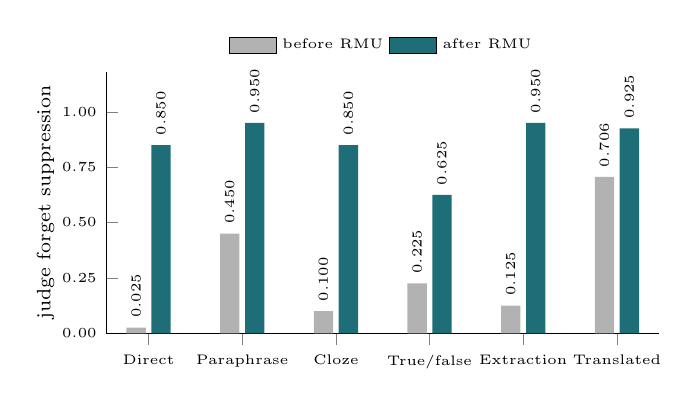
\begin{tikzpicture}
\begin{axis}[
  ybar, bar width=7pt, width=8.6cm, height=4.9cm,
  ymin=0, ymax=1.18, ytick={0,0.25,0.5,0.75,1},
  symbolic x coords={Direct,Paraphrase,Cloze,True/false,Extraction,Translated},
  xtick=data, x tick label style={font=\tiny},
  y tick label style={font=\tiny}, ylabel={\scriptsize judge forget suppression},
  ylabel style={yshift=-4pt},
  nodes near coords, nodes near coords style={font=\fontsize{5}{6}\selectfont,rotate=90,anchor=west},
  yticklabel style={/pgf/number format/precision=2},
  /pgf/number format/.cd, fixed, fixed zerofill, precision=3,
  legend style={font=\tiny,at={(0.5,1.03)},anchor=south,draw=none},
  legend columns=2, enlarge x limits=0.09, axis lines*=left, area legend]
\addplot[fill=beforecol,draw=none] coordinates {(Direct,0.025) (Paraphrase,0.450) (Cloze,0.100) (True/false,0.225) (Extraction,0.125) (Translated,0.706)};
\addplot[fill=aftercol,draw=none] coordinates {(Direct,0.850) (Paraphrase,0.950) (Cloze,0.850) (True/false,0.625) (Extraction,0.950) (Translated,0.925)};
\legend{before RMU, after RMU}
\end{axis}
\end{tikzpicture}\\
{\tiny Global, $n=40$ per format; Translated pools 8 languages ($n=320$). Values from the paper's main table.\par}
\end{column}
\begin{column}{0.40\textwidth}
\scriptsize
\begin{itemize}
\item Injection worked: before RMU the judge sees the fact on 97.5\% of direct questions (suppression 0.025); the base model before injection, on 5\%.
\item After RMU, Wilson 95\% intervals: direct 0.71--0.93; paraphrase and extraction 0.83--0.99; translated 0.89--0.95.
\item Substring recall on direct questions: 0.825 $\to$ 0.000.
\item Translation had little headroom: 0.706 before RMU, so the pooled gain is 0.22.
\item Weakest format: true/false (0.625).
\end{itemize}
\end{column}
\end{columns}
\note{
\begin{itemize}
\item Judge forget suppression on Global rises from 0.025 to 0.85 on direct questions, 0.45 to 0.95 on paraphrases and 0.125 to 0.95 on extraction prompts (n = 40 each), and from 0.706 to 0.925 on the pooled translated prompts (n = 320).
\item Wilson 95\% intervals after RMU, as reported in the paper: 0.71--0.93 (direct), 0.83--0.99 (paraphrase and extraction), 0.89--0.95 (translated). With 40 questions one item moves a rate by 2.5 points.
\item Suppression after RMU is higher on paraphrase and extraction than on direct questions; the paper says this was not expected and is not explained.
\item Cloze 0.100 to 0.850 and true/false 0.225 to 0.625 are split from one 80-item bucket using item-level verdicts.
\item One Global post-RMU translated item was not judged (Hindi, 39 of 40).
\end{itemize}}
\end{frame}

% ======================================================================
\begin{frame}{Results: multilingual leakage (RQ1)}
\begin{columns}[T]
\begin{column}{0.50\textwidth}
\centering
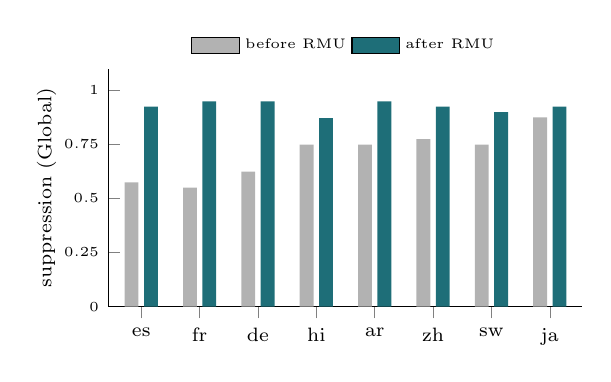
\begin{tikzpicture}
\begin{axis}[
  ybar, bar width=5pt, width=7.6cm, height=4.6cm,
  ymin=0, ymax=1.1, ytick={0,0.25,0.5,0.75,1},
  symbolic x coords={es,fr,de,hi,ar,zh,sw,ja},
  xtick=data, x tick label style={font=\scriptsize},
  y tick label style={font=\tiny}, ylabel={\scriptsize suppression (Global)},
  ylabel style={yshift=-4pt},
  legend style={font=\tiny,at={(0.5,1.02)},anchor=south,draw=none},
  legend columns=2, enlarge x limits=0.08, axis lines*=left, area legend]
\addplot[fill=beforecol,draw=none] coordinates {(es,0.575) (fr,0.550) (de,0.625) (hi,0.750) (ar,0.750) (zh,0.775) (sw,0.750) (ja,0.875)};
\addplot[fill=aftercol,draw=none] coordinates {(es,0.925) (fr,0.950) (de,0.950) (hi,0.872) (ar,0.950) (zh,0.925) (sw,0.900) (ja,0.925)};
\legend{before RMU, after RMU}
\end{axis}
\end{tikzpicture}\\
\tiny es Spanish, fr French, de German, hi Hindi, ar Arabic, zh Chinese, sw Swahili, ja Japanese. Facts injected and unlearned in English only; translations are machine-generated queries.
\end{column}
\begin{column}{0.48\textwidth}
\centering
\tiny
\setlength{\tabcolsep}{3pt}
\begin{tabular}{@{}lcccccc@{}}
\toprule
& \multicolumn{2}{c}{Global} & \multicolumn{2}{c}{Earth} & \multicolumn{2}{c}{Fire}\\
\cmidrule(lr){2-3}\cmidrule(lr){4-5}\cmidrule(lr){6-7}
Lang. & bef. & aft. & bef. & aft. & bef. & aft.\\
\midrule
es & 0.575 & 0.925 & 0.625 & 0.950 & 0.675 & 0.875\\
fr & 0.550 & 0.950 & 0.600 & 0.975 & 0.675 & 0.950\\
de & 0.625 & 0.950 & 0.500 & 0.925 & 0.575 & 0.975\\
hi & 0.750 & 0.872$^\ast$ & 0.700 & 0.875 & 0.850 & 0.825\\
ar & 0.750 & 0.950 & 0.875 & 0.925 & 0.700 & 0.900\\
zh & 0.775 & 0.925 & 0.850 & 0.950 & 0.700 & 0.975\\
sw & 0.750 & 0.900 & 0.725 & 0.950 & 0.675 & 0.925\\
ja & 0.875 & 0.925 & 0.850 & 0.925 & 0.825 & 0.975\\
\bottomrule
\end{tabular}\\[2pt]
{\tiny 40 questions per language. $^\ast$39 of 40 Hindi items judged.}\\[4pt]
\scriptsize
\begin{itemize}
\item Unlearning transferred to all 8 languages: at least 0.87 everywhere except Fire on Hindi (0.825).
\item Hindi is the weakest language after RMU in all three variants.
\end{itemize}
\end{column}
\end{columns}
\note{
\begin{itemize}
\item Forget questions machine-translated into Spanish, French, German, Hindi, Arabic, Chinese, Swahili and Japanese, used only as queries; a native-speaker check of the translations is still pending.
\item English-only unlearning of English-injected facts transferred to all eight languages, with judged suppression after RMU of at least 0.87 everywhere except Fire on Hindi (0.825).
\item Before RMU the injected model already withheld the fact on 71\% of translated prompts (Spanish 0.575, French 0.55, Japanese 0.875 on Global), so headroom is small.
\item In Fire, the South Asian variant, Hindi suppression did not rise (0.850 to 0.825). With one language, 40 questions and one run, the paper does not interpret that.
\item Farashah et al. (Multilingual Amnesia) report mostly language-specific forgetting, but the setups differ: they unlearn in each language with gradient-based objectives on an 8B model.
\end{itemize}}
\end{frame}

% ======================================================================
\begin{frame}{Results: utility cost and format-change leakage (RQ1)}
\begin{columns}[T]
\begin{column}{0.52\textwidth}
\textbf{\small Judged accuracy on non-forget facts}\\[3pt]
\tiny
\setlength{\tabcolsep}{3pt}
\begin{tabular}{@{}lcccccc@{}}
\toprule
& \multicolumn{2}{c}{Global} & \multicolumn{2}{c}{Earth} & \multicolumn{2}{c}{Fire}\\
\cmidrule(lr){2-3}\cmidrule(lr){4-5}\cmidrule(lr){6-7}
& bef. & aft. & bef. & aft. & bef. & aft.\\
\midrule
Retain (64) & 0.516 & 0.422 & 0.562 & 0.516 & 0.531 & 0.500\\
World facts (40/20/20) & 0.875 & 0.850 & 0.900 & 0.900 & 0.900 & 0.900\\
Real authors (40/20/20) & 0.825 & 0.775 & 1.000 & 1.000 & 0.950 & 0.950\\
\bottomrule
\end{tabular}\\[5pt]
\scriptsize
\begin{itemize}
\item Retain falls 9.4 points on Global (Wilson 95\%: 0.40--0.63 before, 0.31--0.54 after), 4.7 on Earth, 3.1 on Fire.
\item Within sampling noise for one variant, but the same sign in all three runs, so we report it as a real cost.
\end{itemize}
\end{column}
\begin{column}{0.46\textwidth}
\textbf{\small Leakage under format change}\\[3pt]
\tiny
\setlength{\tabcolsep}{3pt}
\begin{tabular}{@{}lcccccc@{}}
\toprule
Substring recall & \multicolumn{2}{c}{Global} & \multicolumn{2}{c}{Earth} & \multicolumn{2}{c}{Fire}\\
\midrule
Cloze + T/F pooled & 0.663 & 0.325 & 0.738 & 0.300 & 0.725 & 0.400\\
\bottomrule
\end{tabular}\\[5pt]
\scriptsize
\begin{itemize}
\item Global substring recall after RMU: 0 on direct, paraphrase and extraction; 0.325 on the pooled cloze and true/false (T/F) bucket.
\item Cloze recall is 0 after RMU; T/F carries the leak (substring recall 0.65; judge suppression 0.625).
\item Pooled judge suppression 0.74 (Wilson 95\%: 0.63--0.82); T/F 0.625 (0.47--0.76).
\item No base-model reference on this format.
\end{itemize}
\end{column}
\end{columns}
\note{
\begin{itemize}
\item Utility: judged retain accuracy falls by 9.4 points on Global (0.516 to 0.422; Wilson 95\% intervals 0.40--0.63 before and 0.31--0.54 after, n = 64), 4.7 on Earth and 3.1 on Fire.
\item Global world facts fall 2.5 points and real authors 5.0 points (n = 40 each); Earth and Fire are unchanged on 20 items each.
\item Retain facts were injected only partly (base model 0.0625, after injection 0.516), so the cost is measured on facts the model knew about half the time.
\item Leakage: a true/false (T/F) prompt contains the correct statement, so a model that never learned the fact would accept some of them. Without a base-model reference on this format, we report it as residual leakage, not as a measured amount.
\item Fire's true/false suppression after RMU (0.475) is the lowest cell in the paper's main table.
\end{itemize}}
\end{frame}

% ======================================================================
\begin{frame}{Results: are the facts still decodable? Probes (RQ2)}
\begin{columns}[T]
\begin{column}{0.56\textwidth}
\centering
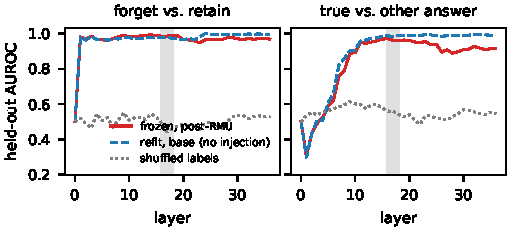
\includegraphics[width=\linewidth]{figures/fig_probe.pdf}\\
{\tiny Held-out probe area under the receiver operating characteristic curve (AUROC) by layer on Global (mean over 5 splits; shaded: update layers 16--18). Left: forget vs.\ retain questions. Right: content probe (true vs.\ other answer). Layer 0 is the embedding output.\par}
\end{column}
\begin{column}{0.42\textwidth}
\scriptsize
\begin{itemize}
\item Logistic probes, scored by held-out AUROC.
\item Forget-vs-retain probes decode at AUROC 0.98 from layer 1 and stay at 0.97--0.99 through layer 36 after RMU.
\item \textbf{But} the base model that never saw the facts does the same: 0.981 (layer 1), 0.977 (layer 16), 0.973 (layer 18). Shuffled labels: 0.46--0.53.
\item Content probe: 0.96 after RMU at layer 18, 0.99 for the base-model refit.
\item \textbf{Reading}: probes reflect surface differences (such as fictitious names), not stored facts. They are uninterpretable as knowledge retention.
\end{itemize}
\end{column}
\end{columns}
\note{
\begin{itemize}
\item At each of the 37 residual positions we take the last non-padding token's activation; a logistic probe separates the 40 forget from the 64 retain questions. Numbers are held out (70/30 split, repeated 5 times on Global, 3 times on Earth and Fire). Metric: area under the receiver operating characteristic curve (AUROC).
\item Frozen probes are fit on the post-injection model and applied after RMU; refit probes are fit on each model's own rows. Controls: base model before injection, and shuffled labels.
\item Earth and Fire agree (base-model refit AUROC 0.994 at layer 1).
\item The probes do not show that facts survive RMU, and a lower score would not have shown erasure. Probes that compare a fact with its counterfactual, with the base-model control, would be needed.
\end{itemize}}
\end{frame}

% ======================================================================
\begin{frame}{Results: relearning test (RQ2)}
\begin{columns}[T]
\begin{column}{0.54\textwidth}
\centering
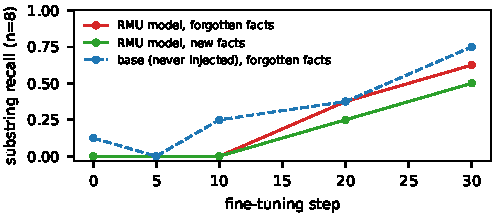
\includegraphics[width=\linewidth]{figures/fig_relearn.pdf}\\
{\tiny Relearning on Global: substring recall on the 8 trained questions at each fine-tuning step.\par}\vspace{4pt}
{\tiny\raggedright Arms: \textbf{RMU-old} = post-RMU model trained on the 8 forgotten facts; \textbf{RMU-new} = same model trained on 8 new fictitious authors; \textbf{Base-old} = never-injected base model trained on the 8 forgotten facts (acquisition reference, not a matched control).\par}
\end{column}
\begin{column}{0.44\textwidth}
\tiny
\setlength{\tabcolsep}{3pt}
\begin{tabular}{@{}lccc@{}}
\toprule
Judge match, step 30 (of 8) & RMU-old & Base-old & RMU-new\\
\midrule
Global, trained & 5 & 7 & 4\\
Earth, trained & 6 & 6 & 5\\
Fire, trained & 6 & 8 & 5\\
Global, held-out paraphrases & 3 & 3 & --\\
Earth, held-out paraphrases & 2 & 4 & --\\
Fire, held-out paraphrases & 6 & 2 & --\\
\bottomrule
\end{tabular}\\[4pt]
\scriptsize
\begin{itemize}
\item Key comparison, RMU-old vs.\ RMU-new on Global: 5/8 vs.\ 4/8, one fact. Wilson 95\%: 0.31--0.86 and 0.22--0.78. Not significant.
\item Base-old reaches 7/8 (0.53--0.98): no savings over learning from scratch.
\item Weak, consistent evidence of residual knowledge at best.
\end{itemize}
\end{column}
\end{columns}
\note{
\begin{itemize}
\item 30 fine-tuning steps (learning rate 2e-4, batch size 1, one run per arm). RMU-old trains the post-RMU model on 8 forgotten facts; RMU-new trains a fresh copy of the same model on 8 new fictitious TOFU authors; base-old trains the never-injected base model on the 8 forgotten facts (an acquisition reference, not a matched control).
\item On Global the RMU model recovers 5 of 8 forgotten facts (from 0 of 8) against 4 of 8 new facts. Earth and Fire show the same one-fact gap (6 against 5) on the same facts, so they are not independent replicates.
\item At step 0 the trained-question counts are 0, 2 and 0 on Global (RMU-old, base-old, RMU-new).
\item Held-out paraphrases are mixed.
\end{itemize}}
\end{frame}

% ======================================================================
\begin{frame}{Judge reliability}
\begin{columns}[T]
\begin{column}{0.52\textwidth}
\scriptsize
\setlength{\tabcolsep}{3pt}
\begin{tabular}{@{}lcccc@{}}
\toprule
Judge agreement & $n$ & raw & $\kappa$ & PABAK / AC1\\
\midrule
Global, base-model pass & 16 & 0.938 & 0.000 & 0.875 / 0.934\\
Global, before RMU & 100 & 0.970 & 0.939 & 0.940 / 0.941\\
Global, after RMU & 99 & 0.929 & 0.829 & 0.859 / 0.880\\
Earth, before + after & 188 & 0.936 & 0.861 & 0.872 / 0.882\\
Fire, before + after & 188 & 0.872 & 0.738 & 0.745 / 0.753\\
\bottomrule
\end{tabular}\\[3pt]
{\tiny \code{qwen3.5:35b} vs.\ Kimi K3 on the seeded 15\% sample. $\kappa$: Cohen's kappa. PABAK: prevalence-adjusted bias-adjusted kappa. AC1: Gwet's first-order agreement coefficient.\par}
\end{column}
\begin{column}{0.46\textwidth}
\scriptsize
\begin{itemize}
\item \textbf{Kappa paradox}: on the base-model pass the judges agree on 15 of 16 items (raw 0.9375), yet $\kappa = 0.0$, because the primary judge never says ``match''. PABAK (0.875) and AC1 (0.934) are insensitive to label prevalence.
\item On evaluation passes $\kappa$ is 0.83--0.94 on Global and 0.74--0.86 on Earth and Fire.
\item Disagreements run one way: on Global all 10 of 199 have the secondary judge saying ``match'' (Earth 9 vs.\ 3, Fire 19 vs.\ 5), so suppression may be overstated by a few points.
\end{itemize}
\end{column}
\end{columns}
\note{
\begin{itemize}
\item The primary judge is qwen3.5:35b (temperature 0, thinking off, JSON verdict); the secondary judge Kimi K3 re-grades a seeded random 15\% sample with the same rubric.
\item We report raw agreement, Cohen's kappa, prevalence-adjusted bias-adjusted kappa (PABAK, 2 times observed agreement minus 1) and Gwet's first-order agreement coefficient (AC1).
\item Kappa becomes unstable when one judge gives almost one label: chance agreement approaches observed agreement. The Earth and Fire base-model passes (16 pairs each) give raw 0.938 and 0.875 with kappa 0.
\item Because disagreements lean one way (primary stricter), primary-judge suppression may be overstated by a few points.
\end{itemize}}
\end{frame}

% ======================================================================
\begin{frame}{Across variants and RMU settings (RQ3)}
\begin{columns}[T]
\begin{column}{0.55\textwidth}
\textbf{\small Judge forget suppression by variant}\\[3pt]
\tiny
\setlength{\tabcolsep}{3pt}
\begin{tabular}{@{}lcccccc@{}}
\toprule
& \multicolumn{2}{c}{Global} & \multicolumn{2}{c}{Earth} & \multicolumn{2}{c}{Fire}\\
\cmidrule(lr){2-3}\cmidrule(lr){4-5}\cmidrule(lr){6-7}
Format ($n$) & bef. & aft. & bef. & aft. & bef. & aft.\\
\midrule
Direct (40) & 0.025 & 0.850 & 0.050 & 0.875 & 0.075 & 0.875\\
Paraphrase (40) & 0.450 & 0.950 & 0.325 & 0.950 & 0.400 & 0.875\\
Cloze (40) & 0.100 & 0.850 & 0.075 & 0.825 & 0.175 & 0.850\\
True/false (40) & 0.225 & 0.625 & 0.175 & 0.625 & 0.075 & 0.475\\
Cloze + T/F pooled (80) & 0.163 & 0.738 & 0.125 & 0.725 & 0.125 & 0.663\\
Extraction (40) & 0.125 & 0.950 & 0.050 & 0.925 & 0.075 & 0.900\\
Translated, 8 langs (320) & 0.706 & 0.925 & 0.716 & 0.934 & 0.709 & 0.925\\
\bottomrule
\end{tabular}\\[3pt]
{\tiny Single run per variant (seed 42).\par}
\end{column}
\begin{column}{0.43\textwidth}
\textbf{\small Masked RMU sweep on Global}\\[3pt]
\tiny
\setlength{\tabcolsep}{3pt}
\begin{tabular}{@{}lcc@{}}
\toprule
Configuration & Suppr. & Retain\\
\midrule
Layer 7, $\alpha=100$, $c=20$ & 1.00 & 0.55\\
Layer 18, $\alpha=50$, $c=20$ & 1.00 & 0.40\\
Layer 18, $\alpha=100$, $c=20$ (main) & 0.85 & 0.45\\
Layer 18, $\alpha=200$, $c=20$ & 0.50 & 0.60\\
Layer 18, $\alpha=100$, $c=40$ & 1.00 & 0.50\\
\bottomrule
\end{tabular}\\[2pt]
{\tiny Seeded subset, 20 forget + 20 retain direct questions; $c$: steering coefficient. Not comparable to the main table.}\\[3pt]
\scriptsize
\begin{itemize}
\item Earth and Fire follow Global within a few points on every format.
\item We do not claim the main configuration is optimal; every masked setting forgot at least partly, unmasked points scored 0.05.
\end{itemize}
\end{column}
\end{columns}
\note{
\begin{itemize}
\item Variants: Earth and Fire follow Global within a few points on every format. Global seeds 43 and 44, Tiny Aya Water, Base and Aya Expanse 8B were queued and did not run in time, so there is no seed spread in this version.
\item Sweep: two configurations scored better than the chosen one on this subset: layer 7 with alpha 100 (1.00 and 0.55) and layer 18 with steering coefficient 40 (1.00 and 0.50). With 20 items per cell one item moves a rate by 5 points, so the subset cannot separate these configurations.
\item The main configuration was fixed before the masked sweep finished. Four earlier unmasked sweep points all scored 0.05, so the mask matters more than the layer on this subset.
\end{itemize}}
\end{frame}

% ======================================================================
\begin{frame}{Limitations}
\footnotesize
\begin{itemize}
\item \textbf{Small samples, one seed}: 40 forget questions from two authors, 64 retain, 20--40 utility questions, relearning on 8 facts per arm, sweep on 20 + 20 items.
\item \textbf{Hyperparameters tuned on the evaluated questions}: $\alpha$ and learning rate were set on the same 40 forget questions.
\item \textbf{Injected facts}: added by an extra fine-tuning phase, which may make unlearning look more resistant than for pretraining knowledge; retain facts injected only partly (0.52).
\item \textbf{English-only injection}, machine-translated queries not yet checked by native speakers.
\item \textbf{Model judges}: disagreements lean one way, so suppression may be overstated by a few points.
\item \textbf{Probes and relearning}: probes may be confounded by topic; relearning uses one schedule, and the base arm is not a matched control.
\item \textbf{Coverage}: Global, Earth and Fire only; general capability is TOFU world\_facts and real\_authors, not broad benchmarks.
\end{itemize}
{\color{stage}\textbf{Bottom line:} consistent with suppression rather than erasure; we do not claim erasure.\par}
\note{
\begin{itemize}
\item Confidence intervals were computed only where stated; seed spread awaits Global seeds 43 and 44.
\item The configuration is not shown to be optimal (see the sweep).
\item English-only injection asks a different question from within-language unlearning.
\item The base model was not evaluated on cloze or true/false prompts, so true/false leakage cannot be separated from accepting a statement placed in the prompt.
\item Water, Base and Aya Expanse 8B did not run; one model family and size.
\item Bottom line from the paper: with a masked forget loss, RMU suppresses the injected facts across three Tiny Aya variants, holding under paraphrase, extraction prompts and translation into eight languages, at a utility cost of 3--9 points on retain facts. It does not establish erasure: format-change leakage lacks a base-model reference, relearning is no faster than learning from scratch, and the RMU-old against RMU-new gap is one fact at n = 8.
\end{itemize}}
\end{frame}

% ======================================================================
\begin{frame}{What's next}
\footnotesize
\textbf{Pending runs}
\begin{itemize}
\item Global seeds 43 and 44 (seed spread), Tiny Aya Water, Base and Aya Expanse 8B.
\item Native-speaker check of the eight-language translations.
\end{itemize}
\textbf{Left to future work}
\begin{itemize}
\item Analysis of the logit-lens, activation-patching and head-ablation artifacts already collected on Global.
\item CircuitKIT EAP-IG circuits: ran on Global, not analyzed in this version.
\item Probes that compare a fact with its counterfactual, together with the base-model control.
\item A base-model reference on cloze and true/false prompts, to measure format-change leakage.
\end{itemize}
\note{
\begin{itemize}
\item Pending from the paper: Global seeds 43 and 44, Water, Base and Aya Expanse 8B, the native-speaker translation check.
\item Logit lens, activation patching, head ablation and CircuitKIT edge attribution patching with integrated gradients (EAP-IG) artifacts exist for Global but are not analyzed in this version; we report nothing from them and leave them to future work.
\item The counterfactual-probe and base-model true/false items come from the paper's discussion and limitations.
\end{itemize}}
\end{frame}

% ======================================================================
\begin{frame}{Links and references}
\small
\begin{itemize}
\item \textbf{Code (GitHub):} \url{https://github.com/mso-docs/Lexsi-Unlearning}
\item \textbf{Adapters, checkpoints, probes, traces (Hugging Face):} dataset \url{https://huggingface.co/datasets/mackenzietechdocs/lexsi-unlearning-eval}; unlearned checkpoints \url{https://huggingface.co/mackenzietechdocs/lexsi-tiny-aya-global-rmu} and Earth, Fire and Water counterparts in the same namespace (CC-BY-NC-4.0, non-commercial).
\item \textbf{Paper:} \url{https://huggingface.co/spaces/mackenzietechdocs/lexsi-unlearning-demo/resolve/main/data/paper/main.pdf}
\end{itemize}
\vspace{4pt}
\scriptsize
\textbf{Key references} (arXiv IDs as listed in the paper):
TOFU (2401.06121); Weapons of Mass Destruction Proxy (WMDP) and RMU (2403.03218); Multilingual Amnesia, Farashah et al.\ (2601.05641); Tiny Aya (2603.11510); LoRA (2106.09685); EAP-IG (2403.17806).\\[4pt]
Built with Lexsi's SafeTune and AuditKIT (CircuitKIT ran; not analyzed in this version). Data: TOFU fictitious authors, no real personal data.
\note{
\begin{itemize}
\item Code, dataset, checkpoints and the paper PDF are linked on this slide. The GitHub repository and Hugging Face artifacts are still private until publication.
\item Releasing checkpoints depends on confirming un-gated republication under the base model's Creative Commons attribution non-commercial (CC-BY-NC) licence and Cohere's acceptable-use policy; gated base weights are not redistributed.
\item Ethics: the forget set is synthetic (TOFU fictitious authors); no real personal data and no hazardous-knowledge data.
\end{itemize}}
\end{frame}

\end{document}
